\chapter {Analýza súčasnej aplikácie}
Táto kapitola sa zaoberá účelom súčasnej aplikácie a analýzou použitých technológií, ktoré sú dôležité pre celkovú funkcionalitu aplikácie. Následne sú popísané technológie, ktoré boli použité pri vývoji súčasnej aplikácie až po podprogramy, ktoré riešia výpočtovo náročnejšie úlohy v rámci tejto aplikácie. Jednému z najdôležitejších podprogramov, \texttt{grid-tracker}, je venovaná väčšia pozornosť. Táto kapitola sa taktiež venuje následnému zostaveniu a spusteniu aplikácie, ktoré je dôležité pre nasledujúcu sekciu, ktorá analyzuje používateľské rozhranie aplikácie.

\section {Účel aplikácie}
Účelom súčasnej aplikácie -- DICOM Viewer -- je analýza pohybu srdcového svalu, pomocou ktorej by bolo možné zistiť anomálie v jeho pohybe. Aplikácia umožňuje importovať súbory typu DICOM (popísaného v sekcii \ref{dicom}), ktoré sú otagované SPAMM mriežkou.

Na importovaných snímkach je následne používateľom vytvorená mriežka, ktorej parametre môžu byť následne používateľom upravené. Štruktúra a parametre týchto mriežok sú neskôr poslané podprogramu \texttt{grid-tracker}, ktorého úlohou je zarovnanie používateľom vytvorených mriežok s mriežkami vytvorenými SPAMM technikou. Po ich zarovnaní je možné pomocou techniky grafových rezov odsegmentovať srdečné komory a tým pádom zúžiť analýzu pohybu srdcového svalu len na tieto komory.

Cieľom tejto diplomovej práce je vytvorenie webovej verzie súčasnej aplikácie vrátane zarovnania mriežok pomocou \texttt{grid-tracker} podprogramu (\ref{helper_apps}).

\section {Použité technológie}
Popisu použitých technológií v súčasnej desktopovej aplikácii sa venuje táto sekcia. Na základe zistenia, aké technológie a aplikačné závislosti aplikácia využíva, bude nakoniec možné aplikáciu zostaviť a vyskúšať. Nasledujúci prehľad použitých technológií je založený na dôslednom preskúmaní zdrojového kódu aplikácie, ktorý sa vyznačoval skoro neexistujúcou dokumentáciou. Bez tejto dokumentácie bola orientácia v zdrojovom kóde náročnejšia, čoho dôsledkom bolo predĺženie času potrebného pre analýzu celkovej architektúry súčasnej aplikácie.

\subsection {Qt}
Súčasná aplikácia bola vyvinutá pomocou Qt\footnote{https://www.qt.io/product/qt6} -- cross-platformového frameworku určeného pre vytváranie aplikácií najmä v jazyku C\texttt{++}\footnote{https://isocpp.org}. Aplikácie vyvinuté týmto frameworkom majú výhodu v tom, že sú spustiteľné na rôznych operačných systémoch s minimálnym počtom zmien v zdrojovom kóde \cite{qt_description} (vlastný preklad). V súčasnosti (od roku 2014) zastrešuje vývoj tohto frameworku spoločnosť The Qt Company.

Výsadou Qt frameworku je taktiež rozdelenie jeho funkcionality do jednotlivých modulov. Pri následom vytváraní aplikácie sa použijú len také moduly, ktoré sú v danej aplikácii potrebné \cite{qt_description} (vlastný preklad).

Existujúca aplikácia využíva tento framework vo verzii 5.15, ktorá sa vyznačuje tým, že je to verzia s dlhodobou podporou. Koniec podpory tejto verzie je naplánovaný na 26.5.2023. Najnovšia verzia Qt frameworku je momentálne verzia 6.5, ktorá je zároveň verziou s dlhodobou podporou.

Čo sa týka súčasnej desktopovej aplikácie, v nej boli použité nasledovné moduly: 

\begin{itemize}
\item {Qt Core}
\item {Qt Widgets}
\item {Qt GUI}
\item {Qt Test}
\end{itemize}

Qt Core\footnote{https://doc.qt.io/qt-5/qtcore-index.html} modul obsahuje najpoužívanejšie triedy ako napr. \texttt{QCoreApplication}, \texttt{QObject}, \texttt{QDebug} a iné. Nakoľko sú tieto triedy používané aj inými modulmi, je tento modul implicitne nalinkovaný Qt frameworkom pri budovaní aplikácie \cite{qtcore_description} (vlastný preklad). \newline

Qt Widgets\footnote{https://doc.qt.io/qt-5/qtwidgets-index.html} modul poskytuje UI elementy, ktoré sú určené pre vytváranie používateľského rozhrania. Tieto elementy môžu zobrazovať rozličné dáta, prijímať vstup z klávesnice, byť štylizované a zoskupované do rozličných usporiadaní \cite{qtwidgets_description} (vlastný preklad). Existujúca aplikácia používa z modulu napr. triedu \texttt{QMainWindow}, ktorá je zodpovedná za vykreslenie aplikačného okna a taktiež triedu \texttt{QGraphicsScene}, ktorá je zodpovedná za vykreslenie snímkov z magnetickej rezonancie v DICOM formáte. \newline

Qt GUI\footnote{https://doc.qt.io/qt-5/qtgui-index.html} modul obsahuje triedy určené pre zobrazovanie aplikačného okna a iného grafického obsahu s následnou obsluhou udalostí. Taktiež obsahuje triedy, ktoré sú zodpovedné za zobrazovanie 2D grafiky, fontov a typografie \cite{qtgui_description} (vlastný preklad).
Súčasná aplikácia z tohto modulu používa napr. triedu \texttt{QImage}, ktorá obsahuje metódy pre priamy prístup k pixelom snímkov a ich manipuláciu. \newline

Qt Test\footnote{https://doc.qt.io/qt-5/qttest-index.html} modul poskytuje rozličné triedy pre jednotkové testovanie Qt aplikácií a príslušných knižníc \cite{qttest_description} (vlastný preklad) -- v súčasnej aplikácii bol tento modul využitý pri testovaní grafického používateľského rozhrania a funkcionalít súčasnej aplikácie, ako napr. testovanie zmien v nastaveniach vykreslenej mriežky na obrázku z magnetickej rezonancie.

\subsection {Qmake}\label{qmake}
Pre zjednodušenie písania Makefilov, ktoré definujú, ako má byť program skompilovaný, bol použitý nástroj Qmake\footnote{https://doc.qt.io/qt-5/qmake-manual.html}. Tento nástroj pochádza taktiež z dielne The Qt Company. Qmake umožňuje vývojárom definovať vytváranie rozličných Makefilov pre daný program pomocou syntaxu definovaného programom Qmake \cite{qmake_description} (vlastný preklad). Výsledkom tohto procesu je súbor s príponou \texttt{.pro} obsahujúci inštrukcie, ako daný Makefile vytvoriť. Následne sa pomocou príkazu \texttt{qmake} s argumentom cesty k \texttt{.pro} súboru vytvorí \texttt{Makefile} súbor, pomocou ktorého je možné daný program skompilovať, čoho výsledkom je spustiteľný súbor aplikácie.

Pre súčasnú aplikáciu sa daný súbor volá \texttt{Cameo.pro} a nachádza sa v adresári \texttt{dicomViewer}.

\subsection {DICOM}\label{dicom}
V súčasnosti sú snímky získané pomocou zobrazovacích techník v medicíne zväčša ukladané v archivačnom a komunikačnom systéme snímkov. Tento systém ukladá nielen snímkové dáta ale aj iné relevantné dáta k týmto snímkam podľa štandardu známom ako DICOM\footnote{https://www.dicomstandard.org} (Digital Imaging and Communications in Medicine) \cite{Varma_2012} (vlastný preklad). Ten je medzinárodným štandardom pre komunikáciu a manažment informácií o medicínskych obrazových a k nim príslušných dátach. Definuje, ako majú byť takéto dáta spracovávané, ukladané, tlačené a prenášané medzi zariadeniami podporujúcimi príjem týchto dát \cite{about_dicomlibrary} (vlastný preklad).

Začiatok vývoja DICOM štandardu sa datuje k prelomu 80. a 90. rokoch 20. storočia, kedy započala spolupráca medzi American College of Radiology a National Electrical Manufacturers Association. NEMA taktiež vlastní autorské práva k tomuto štandadu. Momentálne sa DICOM skladá z 22 nezávislých častí, z ktorých avšak nie všetky musia byť implementované daným zariadením podporujúcim tento štandard \cite{dicom_history} (vlastný preklad).

Pre účely spracovania snímkových dát, DICOM štandard vo svojej 10. časti definuje dátovú štruktúru (formát) súboru, do ktorého sa tieto dáta ukladajú. Dátová štruktúra súboru, ktorý spĺňa podmienky 10. časti tohto štandaru, býva značená ako \uv{DICOM Part 10} súbor, inak známy ako DICOM súbor \cite{Varma_2012} (vlastný preklad).

Štruktúra tohto (binárneho) súboru je nasledovná -- prvých 128 bajtov býva zväčša prázdnych (vyplnených 0). Ďalšie 4 bajty obsahujú uložený reťazec \uv{DICM}.  Na základe týchto bajtov sa dá určiť, či sa jedná alebo nejedná o DICOM súbor.
Ďalej nasleduje hlavička, ktorá je rozdelená na viacero skupín zoskupujúcich súvisiace atribúty. Konkrétne atribúty sa adresujú tagom - ten sa skladá z 8 čísiel v hexadecimálnom formáte. Prvé 4 čísla reprezentujú skupinu, v ktorej sa daný atribút nachádza a posledné 4 čísla jednoznačne identifikujú konkrétny atribút v skupine \cite{Varma_2012} (vlastný preklad).

Ako príklad bude uvedené získanie informácie o pacientovom veku - všetky informácie o pacientovi sa nachádzajú v skupine 0010. Pacientov vek v tejto skupine sa nachádza na pozícii 1010, tým pádom výsledný tag pod ktorým nájdeme vek pacienta je (0010, 1010). Ku každému tagu je jednoznačne priradená reprezentácia jej hodnoty, ktorý určuje dátový typ, formát a dĺžku hodnoty daného atribútu  \cite{Varma_2012} (vlastný preklad).

Po hlavičke nasleduje skupina 7FE0, ktorá už obsahuje dáta o samotných obrazových pixeloch \cite{Varma_2012} (vlastný preklad). Typ kódovania týchto dát určuje Transfer Syntax -- ten udáva, akým spôsobom sú obrazové pixely zakódované. Transfer Syntax obsahuje taktiež informáciu, v akom poradí bajtov sú informácie zakódované (Little Endian vs Big Endian) a aká kompresia obrazových dát bola použitá \cite{dicom_transfer_syntax} (vlastný preklad).

\subsection {DCMTK}\label{dcmtk}
DCMTK\footnote{https://dicom.offis.de/en/dcmtk/dcmtk-tools/} je knižnica, ktorá implementujú veľkú časť DICOM štandardu v jazykoch C a C\texttt{++}. Úlohou tejto knižnice je okrem iného skúmanie, vytváranie a konverzia DICOM súborov, manipulácia s pamäťovými médiami a odosielanie, resp. prijímanie obrazových súborov cez internetové pripojenie. Za jej vývojom stojí nemecká firma OFFIS, ktorá túto knižnicu vyvíja nepretržite už od roku 1993. V súčasnosti sa používa v nemocniciach a rôznych spoločnostiach po celom svete, kde predstavuje softvérový základ pri rozličných výskumných projektoch, prototypoch a komerčných produktoch nevynímajúc \cite{dcmtk_description} (vlastný preklad). \newline

Súčasná aplikácia je kompatibilná s najnovšou verziou tejto knižnice, ktorou je verzia 3.6.7. DCMTK knižnica je v tejto aplikácii použitá pre získanie informácií z hlavičiek DICOM súborov, ako napr:

\begin{itemize}
\item {údaje o pacientovi,}
\item {údaje o snímku a}
\item {údaje o sérií snímkov.}
\end{itemize}

\subsection {OpenMP}\label{openmp}
OpenMP\footnote{https://www.openmp.org} poskytuje rozhranie pre programovanie aplikácií (tzv. API), vďaka ktorému je možné vytvárať C\footnote{https://www.open-std.org/jtc1/sc22/wg14/}, C\texttt{++} a Fortran\footnote{https://fortran-lang.org/en/} aplikácie využívajúce viac vlákien nad zdieľanou pamäťou. Vývoj OpenMP v súčasnosti zastrešuje \newline OpenMP Architecture Review Board.
OpenMP funguje na báze direktív, pomocou ktorých sa jednotlivé časti programu dajú paralelizovať viacerými spôsobmi -- a to paralelizáciou prevádzania jednotlivých úloh (tzv. funkčný paralelizmus -- vhodný pre paralelizáciu rekurzívnych algoritmov, kde úloha = volanie funkcie) alebo paralelizáciou dátovo nezávislých for loop iterácií (tu sa jedná o tzv. iteračný dátový paralelizmus) \cite{openmp_description}.

Existujúca aplikácia využíva direktívy OpenMP pre paralelizáciu výpočetne náročnejších algoritmov. Súčasná verzia OpenMP, verzia 5.2, je plne kompatibilná s aktuálnym zdrojovým kódom aplikácie.

\subsection {TNL}\label{tnl}
Template Numerical Library\footnote{https://tnl-project.org} je numerická knižnica, ktorá poskytuje rozličné dátové štruktúry, ktoré uľahčujú prácu s pamäťou a vývoj efektívnych numerických riešičov. Táto knižnica je implementovaná pomocou C\texttt{++} s cieľom poskytnúť flexibilné a užívateľsky prívetivé rozhranie. TNL poskytuje natívnu podporu pre moderné hardwarové architektúry ako sú viacjadrové CPU, GPU a distribuované systémy, ktoré je možné spravovať cez jednotné rozhranie \cite{tnl_description}.

Vývoj TNL knižnice od jej počiatku riadi Tomáš Oberhuber z Katedry matematiky na FJFI ČVUT v spolupráci s Jakubom Klinkovským a Alešom Wodeckim.

V súčasnej aplikácii sú z TNL knižnice použité kolekcie ako napr. \texttt{String} pre manipuláciu s reťazcami a \texttt{Containers::Array}, \texttt{Containers::\{Vector,\newline StaticVector,MultiVector\}}, čo sú šablóny pre reprezentáciu \newline n-dimenzionálnych polí, ktoré abstrahujú manažment dát a exekúciu bežných operácií na rozličných hardvérových architektúrach.

Aplikácia z TNL knižnice taktiež používa \texttt{Solvers::ODE::Merson} -- jedná sa o Runge-Kutta-Merson metódu štvrtého rádu s adaptívnym výberom časového kroku, pomocou ktorej vieme získať približné riešenie diferenciálnych rovníc.

Bohužiaľ, súčasná aplikácia nie je kompatibilná s najnovšími zdrojovými kódmi TNL knižnice -- pre nájdenie posledného \uv{dobrého stavu} knižnice, t.j. stavu za ktorého bolo možné aplikáciu skompilovať, bol využitý nástroj \texttt{git bisect}. Tento nástroj našiel ako posledný \uv{dobrý stav} knižnice z 13.5.2021. Pri využití TNL knižnice zostavenej po tomto dátume nebolo možné súčasnú aplikáciu skompilovať.

\section {Pomocné podprogramy}\label{helper_apps}
Súčasná aplikácia obsahuje a využíva nasledujúce 3 podprogramy:

\begin {itemize}
\item {grid-tracker}
\item {local-variance}
\item {graph-cuts}
\end {itemize}

\texttt{grid-tracker} C\texttt{++} podprogram určený pre sledovanie pohybu myokardu pomocou detekcie SPAMM mriežky z DICOM snímku a mriežky vytvorenej používateľom. Mriežku vytvorenú používateľom sa snaží zarovnať so SPAMM mriežkou pre každú snímku zo sekvencie snímkov. Výstupom sú upravené koordináty bodov mriežky vytvorenej používateľom -- tie sa následne aplikujú namiesto doterajšej mriežky, čoho výsledkom je zobrazenie mriežky s upravenými koordinátmi bodov. \newline

Vstupom tohto programu sú nasledujúce parametre:
\begin {itemize}
\item {\texttt{inputImageFileNames} -- vektor reťazcov reprezentujúce cesty k súborom multivektorov (definované TNL knižnicou), ktoré obsahujú enkódované DICOM snímky,}
\item {\texttt{inputGridFileNames} -- vektor reťazcov reprezentujúce cesty k súborom používateľom definovaných mriežok uložených ako TNL textový multivektor,}
\item {\texttt{outputGridFileNames} (nepovinné)-- vektor reťazcov reprezentujúce cesty k súborom spracovaných mriežok, ktoré budú uložené ako textový TNL multivektor,}
\item {\texttt{curvatureCoefficient} -- závislosť vývoja mriežky od zakrivenia, vyššie číslo znamená vyššiu závislosť,}
\item {\texttt{forceCoefficient} -- závislosť mriežky od gradientu obrazu, vyššie číslo znamená vyššiu závislosť,}
\item {a \texttt{stopTime} -- časový interval algoritmického výpočtu.}
\end {itemize}

Pre daný výpočet \texttt{grid-tracker} využíva technológie \nameref{tnl} a \nameref{openmp}.

Jeho výstupom sú predchádzajúce používateľom definované mriežky v textovom TNL multivectore upravené algoritmom tak, aby mriežky zodpovedali mriežkam definovanými SPAMM metódou. \newline

Nasledujúce dva C\texttt{++} podprogramy nie sú dôležité pre túto diplomovú prácu, avšak pre úplnosť je ich účel vysvetlený. \newline

Úlohou \texttt{local-variance} podprogramu je aplikovanie filtra lokálnej variancie pre danú snímku za účelom neskoršej lepšej segmentácie srdcových komôr. Tento filter je implentovaný pomocou jednoduchého rozptylového filtru, ktorý vypočíta priemernú intenzitu pixelov vo štvorcovom okolí každého pixelu a túto hodnotu dosadí do výberového rozptylu, ktorý sa bude rovnať novej hodnote intenzity pixelu \cite{master_thesis_app}.

Podprogram \texttt{graph-cuts} slúži pre segmentáciu srdcových komôr, ktorá vychádza z predpokladu, že hranica medzi objektom a jeho pozadím sa nachádza v miestach nekonzistencie susedných pixelov snímky. Implementovaná metóda, ktorá dosiahla dobré výsledky bola metóda grafových rezov, kombinujúca Fordov-Fulkersonovým algoritmom s Preflow-Push algoritmom \cite{master_thesis_app}.

\section {Zostavenie aplikácie a jej spustenie}
Pre potrebu popísania používateľského rozhrania je najprv žiaduce dosiahnuť zostavenie existujúcej aplikácie a jej následné spustenie. Po počiatočnej analýze zdrojového kódu, v ktorom bolo zistené, že aplikácia bola vyvíjaná pre Linuxové prostredie, bol vo virtuálnom prostredí nainštalovaný operačný systém Ubuntu 22.10\footnote{https://ubuntu.com}.

Pre zostavenie súčasnej aplikácie bude potrebné nainštalovať Qt framework spolu s nástrojom Qmake, nakoľko ich architektúra súčasnej aplikácia vyžaduje.

Pre inštaláciu Qmake nástroja je potrebné nainštalovať balíček \texttt{qt5-default}\footnote{sudo apt install qt5-default}. Ten obsahuje nie len nástroj \texttt{qmake} ale aj aplikáciu Qt Creator\footnote{https://doc.qt.io/qtcreator/}.

Qt Creator je aplikácia, ktorá poskytuje prostredie pre integrovaný vývoj aplikácií postavených nad Qt frameworkom. Pomocou tejto aplikácie je možné vyvíjať, testovať, zostavovať, spúšťať a debugovať aplikácie postavené na tomto frameworku. Táto aplikácia bude neskôr využitá pre neskorší debugging súčasnej aplikácie.

Okrem balíčku \texttt{qt5-default} je taktiež potrebné nainštalovať balíčky \texttt{cmake}\footnote{sudo apt install cmake} a \texttt{build-essential}\footnote{sudo apt install build-essential}, čo sú balíčky poskytujúce ďalšie nástroje potrebné pre úspešné zostavenie aplikácie. Tieto balíčky v niektorých prípadoch už môžu byť súčasťou použitej linuxovej distribúcie, čo ale neplatilo v prípade použitia Ubuntu 22.10 ako operačného systému.

Pretože súčasná aplikácia využíva DCMTK knižnicu, ako bolo popísané v sekcii \ref{dcmtk}, je tiež nutné nainštalovať nasledujúce balíčky: \texttt{dcmtk}\footnote{sudo apt install dcmtk} \newline a {\texttt{libdcmtk-dev}\footnote{sudo apt install libdcmtk-dev}.

Prvý z uvedených balíčkov nainštaluje samotnú DCMTK knižnicu, druhý obsahuje knižnice a hlavičkové súbory pre vývoj aplikácií používajúce túto knižnicu. Nakoľko v \texttt{Dicom.pro} súbore (ktorý je určený pre výsledné zostavenie aplikácie) sa nachádzajú cesty ku knižniciam z balíčku \texttt{libdcmtk-dev}, je aj tento balíček nutný nainštalovať pre neskoršie korektné spustenie súčasnej aplikácie.

Keďže \texttt{grid-tracker} podprogram obsahuje OpenMP direktívy pre paralelizáciu výpočetných algoritmov, je potrebné nainštalovať OpenMP prostredníctvom balíčku \texttt{libomp-dev}\footnote{sudo apt install libomp-dev}. TNL knižnica bude taktiež benefitovať z inštalácie tohto balíčka, nakoľko sama využíva OpenMP pre paralelizáciu algoritmov, čo znamená, že sa tento balíček nainštaluje ešte pred samotnou inštaláciou TNL knižnice.

Ďalej je potrebné nainštalovať samotnú TNL knižnicu -- pre jej inštaláciu bude potrebné stiahnuť zdrojové kódy buď formou zabaleného zdrojového kódu v .zip balíčku, alebo naklonovaním repozitára pomocou programu \texttt{git}\footnote{https://git-scm.com}. Keďže aplikácia je nekompatibilná s najnovšou verziou TNL knižnice, je potrebné stiahnuť alebo naklonovať repozitár so zdrojovými kódmi do dátumu 13.5.2021 (viď \ref{tnl}).

Nakoľko je nutné samotnú knižnicu zo zdrojových kódov zostaviť, je nevyhnutné mať nainštalovaný kompilátor podporovaný samotnou knižnicou. Medzi podporované kompilátory sa radí GCC\footnote{http://gcc.gnu.org} kompilátor vo verzii 8.0 a vyššie alebo Clang\footnote{https://clang.llvm.org} vo verzii 7.0 a vyššie. Prvý z nich je možné nainštalovať pomocou balíčku \texttt{gcc}\footnote{sudo apt install gcc} a druhý pomocou balíčku \texttt{clang}\footnote{sudo apt install clang}.

Následne je potrebné exekuovať inštalačný skript \texttt{install}, ktorého účelom je nakonfigurovanie TNL knižnice a jej zostavenia.
Pred exekuovaním samotného inštalačného skriptu \texttt{install} je potrebné zistiť, či sú nainštalované balíčky \texttt{doxygen}\footnote{https://doxygen.nl/index.html}, \texttt{matplotlib}\footnote{https://matplotlib.org} a \texttt{graphviz}\footnote{https://graphviz.org}. Tieto balíčky sa využívajú pri generovaní dokumentácie počas exekúcie \texttt{install} skriptu (pri defaultnej inštalácii). Ak sa niektorý z daných balíčkov nenachádza v systéme, je potrebné ho doinštalovať.

Po nainštalovaní všetkých potrebných balíčkov nastal čas pre zostavenie TNL knižnice spustením \texttt{install}\footnote{chmod +x install \&\& ./install} skriptu. Po jeho ukončení sa hlavičkové súbory TNL knižnice budú nachádzať v priečinku \texttt{/usr/lib/aarch64-linux-gnu}. Názov posledného priečinku sa môže líšiť, nakoľko je závislý na architektúre CPU, na ktorom sa TNL knižnice zostavuje. V tomto prípade bola knižnica zostavovaná na systéme Ubuntu 22.10 bežiacom nad CPU s architektúrou Aarch64 (Apple M1 Pro CPU).

Ďalším krokom pre úspešné zostavenie aplikácie je definovanie cesty k hlavičkovým súborom TNL knižnice v samotnom \texttt{Cameo.pro} súbore, určenom pre zostavenie aplikácie pomocou programu \texttt{qmake}. Po otvorení súboru \texttt{Cameo.pro} je teda potrebné nastaviť hodnotu premennej \lstinline{DCMTK_LIBS} -- v tomto prípade ju bolo potrebné nastaviť na \texttt{/usr/lib/aarch64-linux-gnu} a následne daný súbor uložiť.

Po prevedení všetkých predchádzajúcich krokoch je možné spustiť nástroj \texttt{qmake} pomocou krokov popísaných v sekcii \ref{qmake}. Jeho výsledkom bude \newline \texttt{Makefile} súbor, ktorý definuje kroky, ako zostaviť súčasnú aplikáciu. V tomto momente je už možné súčasnú aplikáciu skompilovať pomocou spustenia príkazu \texttt{make install}.

Po skompilovaní aplikácie sa v rovnakom priečinku objaví spustiteľný súbor \texttt{Cameo}, ktorému je potrebné nastaviť práva pre spustenie príkazom \texttt{chmod +x Cameo}. Následne je možné spustiť aplikáciu príkazom \texttt{./Cameo}. \clearpage

\section {Používateľské rozhranie}\label{old_ui}
Po úspešnom spustení aplikácie sa používateľovi zobrazí hlavné okno aplikácie.
V aplikačnom okne sa taktiež zobrazí menu s nasledovnými možnosťami:

\begin {enumerate}
\item {File}
	\begin {enumerate}
		\item {Open -- otvorí systémové okno pre výber priečinku s DICOM snímkami, ktoré sa majú importovať do aplikácie}
		\item {Save Image}
		\begin {enumerate}
			\item {Save View -- uloží pohľad na aktuálnu snímku vo zvolenom formáte}
			\item {Save Scene -- uloží scénu vo zvolenom formáte}
			\item {Save Area of Interes [sic] -- uloží plochu záujmu vo zvolenom formáte}
		\end {enumerate}
	\item {Save all selected}
		\begin {enumerate}
			\item {Save View -- uloží pohľad vybraných snímky vo zvolenom formáte}
			\item {Save Scene -- uloží scénu vybraných snímkov vo zvolenom formáte}
			\item {Save Area of Interes [sic] -- uloží plochu záujmu vybraných snímkov vo zvolenom formáte}
		\end {enumerate}	
	\item {Exit -- ukončí aplikáciu}
	\end {enumerate}
\item {Aditional [sic] Tools}
	\begin {enumerate}
	\item {Grid Tools -- otvorí ľavý postranný panel aplikácie s nastavením mriežky}
	\item {Lvf Tools -- otvorí ľavý postranný panel aplikácie s nastavením filtru lokálnej variácie}
	\item {Graph Cuts Tools -- otvorí ľavý postranný panel aplikácie s nastavením grafových rezov}
	\end {enumerate}
\item {Help}
	\begin {enumerate}
	\item {About -- zobrazí informácie o DICOM Viewer aplikácii}
	\end {enumerate}
\end {enumerate}

Po spustení sa aplikácia nachádza v stave, v ktorom nie je možné s ňou interagovať -- inými slovami, je najprv potrebné do aplikácie importovať snímky v DICOM formáte, ako je ukázané na nasledujúcom obrázku.

\clearpage

\begin {center}
        \centering
        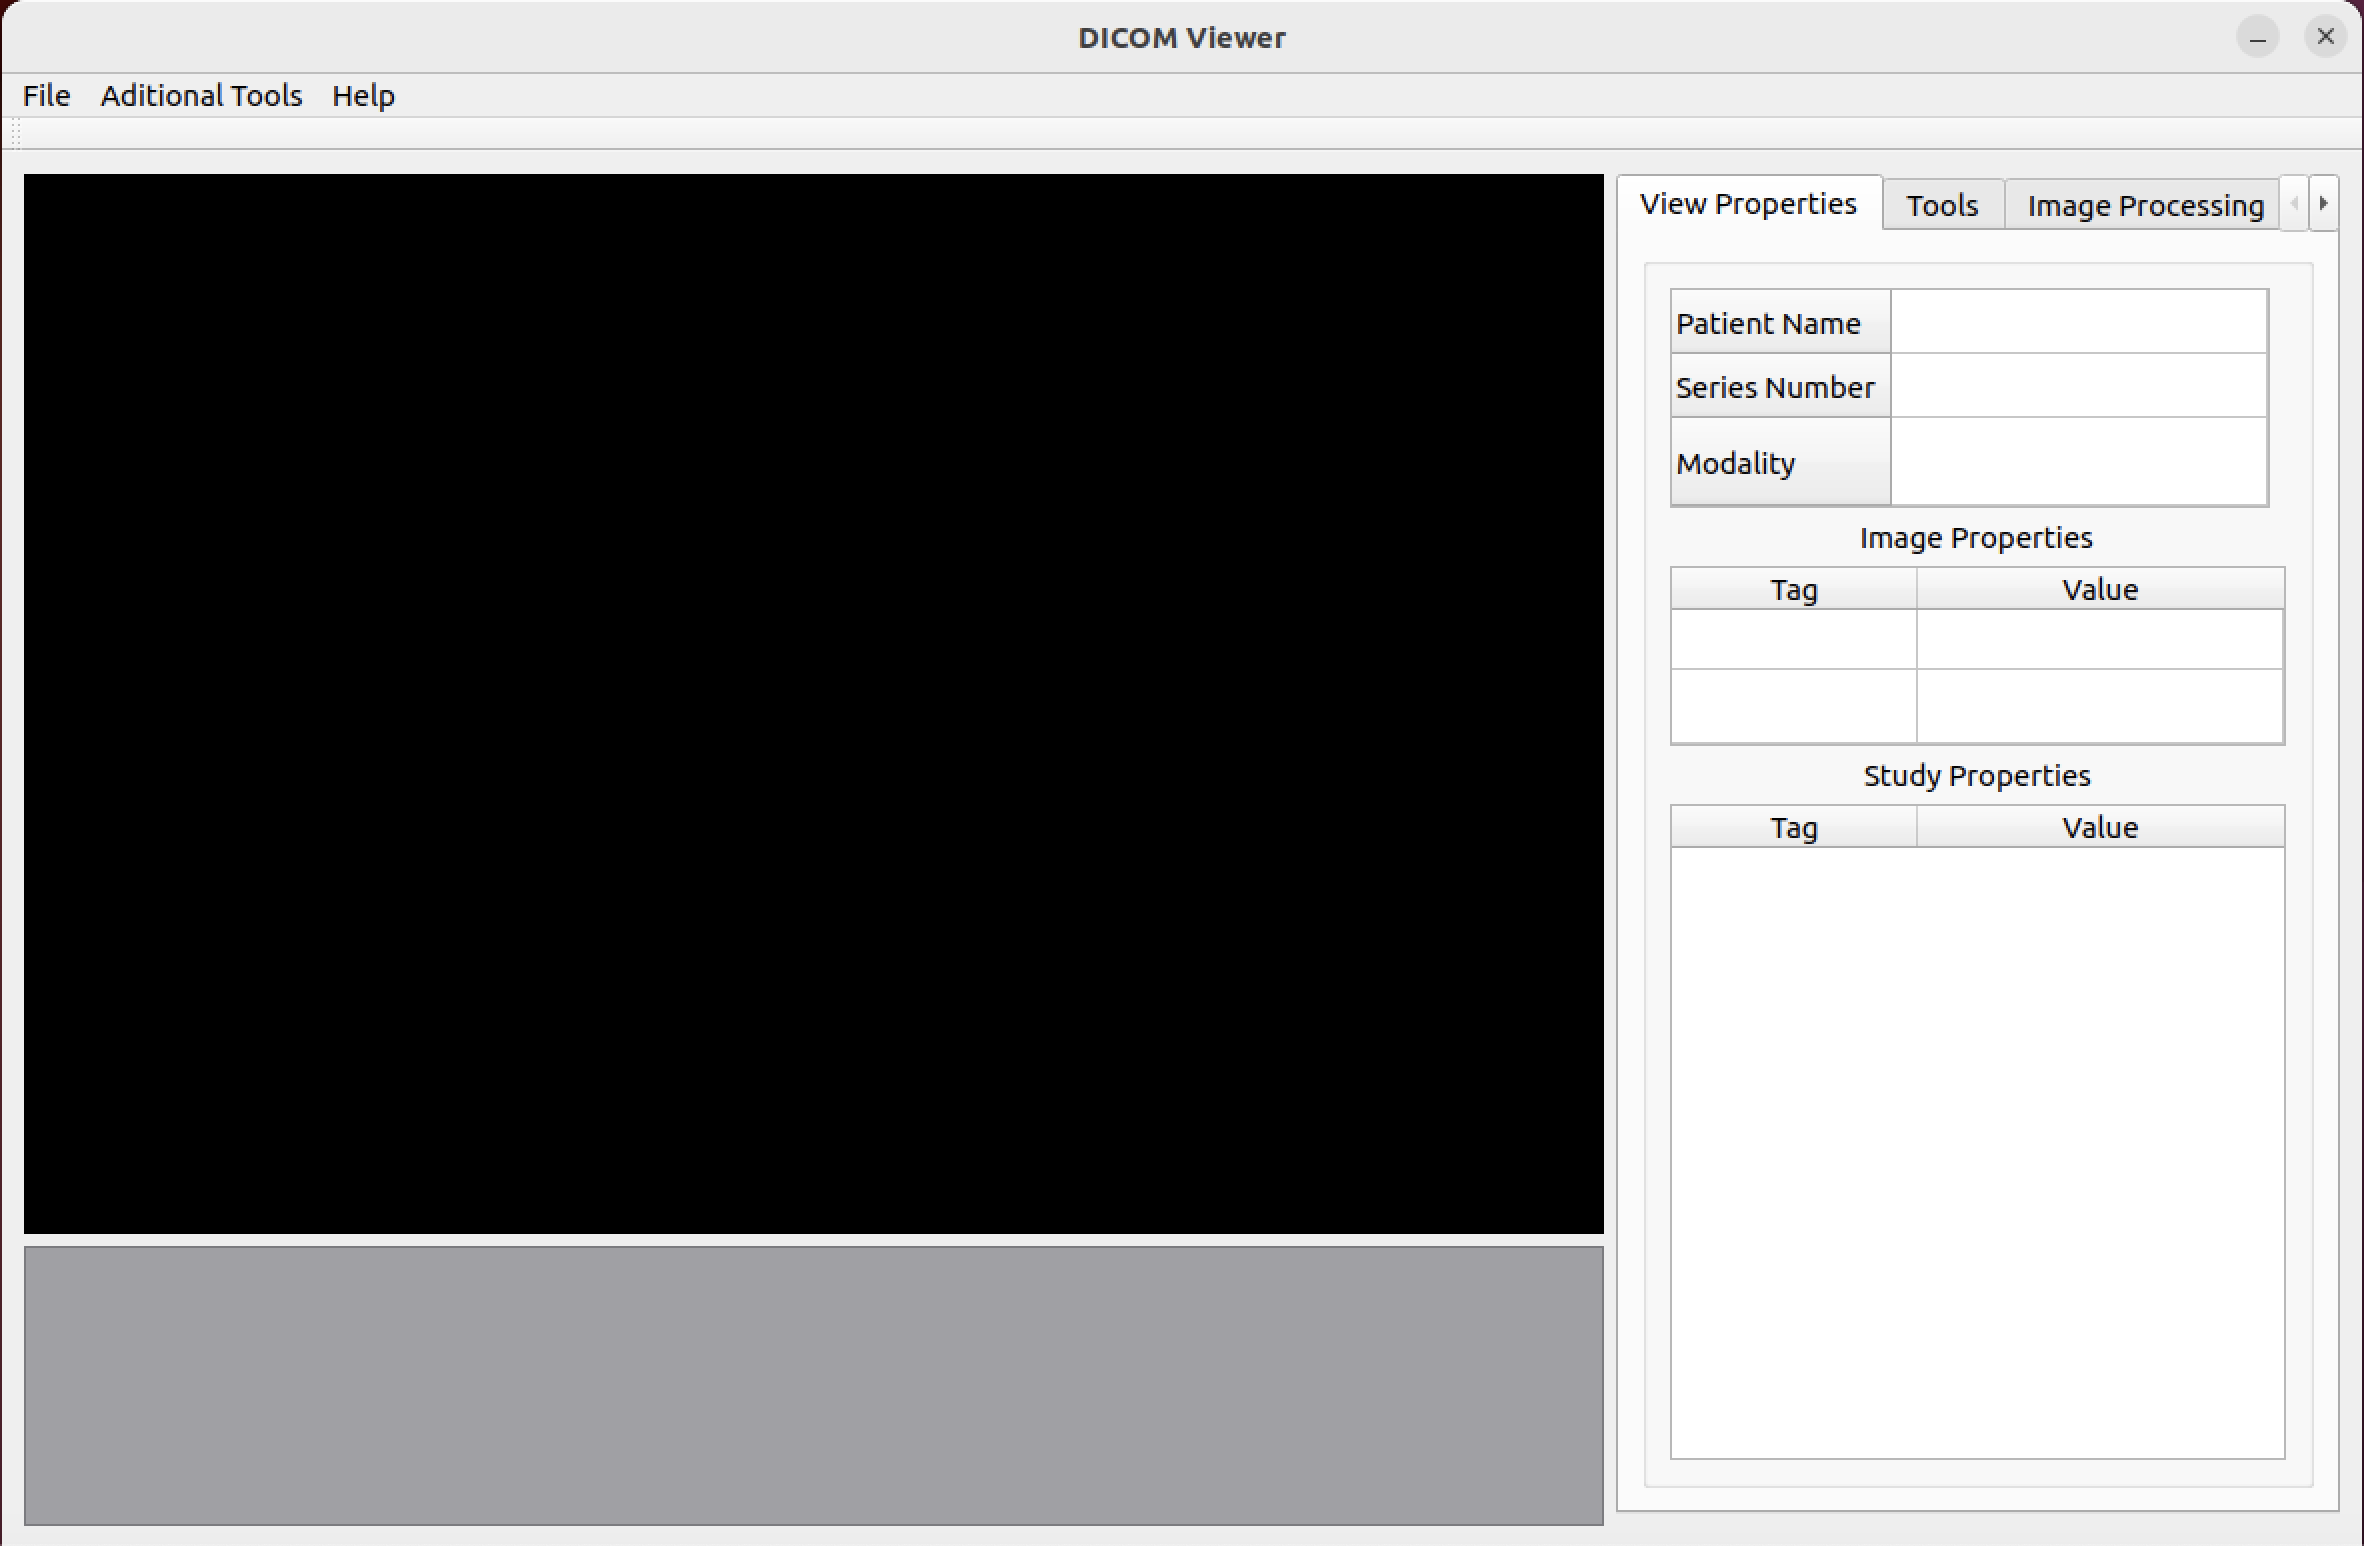
\includegraphics[height=7cm]{media/existing_app/init.png}
        \captionsetup{justification=centering}
        \captionof{figure}[Ukážka DICOM Viewer aplikácie po spustení]{Ukážka DICOM Viewer aplikácie po spustení}
\end {center}

To sa docieli pomocou zvolenia možnosti File $\rightarrow{ Open}$ z aplikačného menu. Následne sa otvorí systémové okno pre výber priečinka s DICOM snímkami, ktoré sa majú zobraziť v aplikácii. Bohužiaľ, nie je možné zvoliť snímky jednotlivo z priečinku, čo zapríčiní načítanie všetkých snímok z daného priečinku do aplikácie. Po zvolení priečinku sa zobrazí prvý snímok v aplikácii. Po výbere ľubovolnej možnosti, ktoré ponúka Aditional [sic] Tools menu, sa taktiež zobrazí ľavý postranný panel v aplikácii, ako je možné vidieť na snímke aplikácie nižšie. V tomto prípade bola zvolená možnosť \uv{Grid Tools}.

\begin {center}
        \centering
        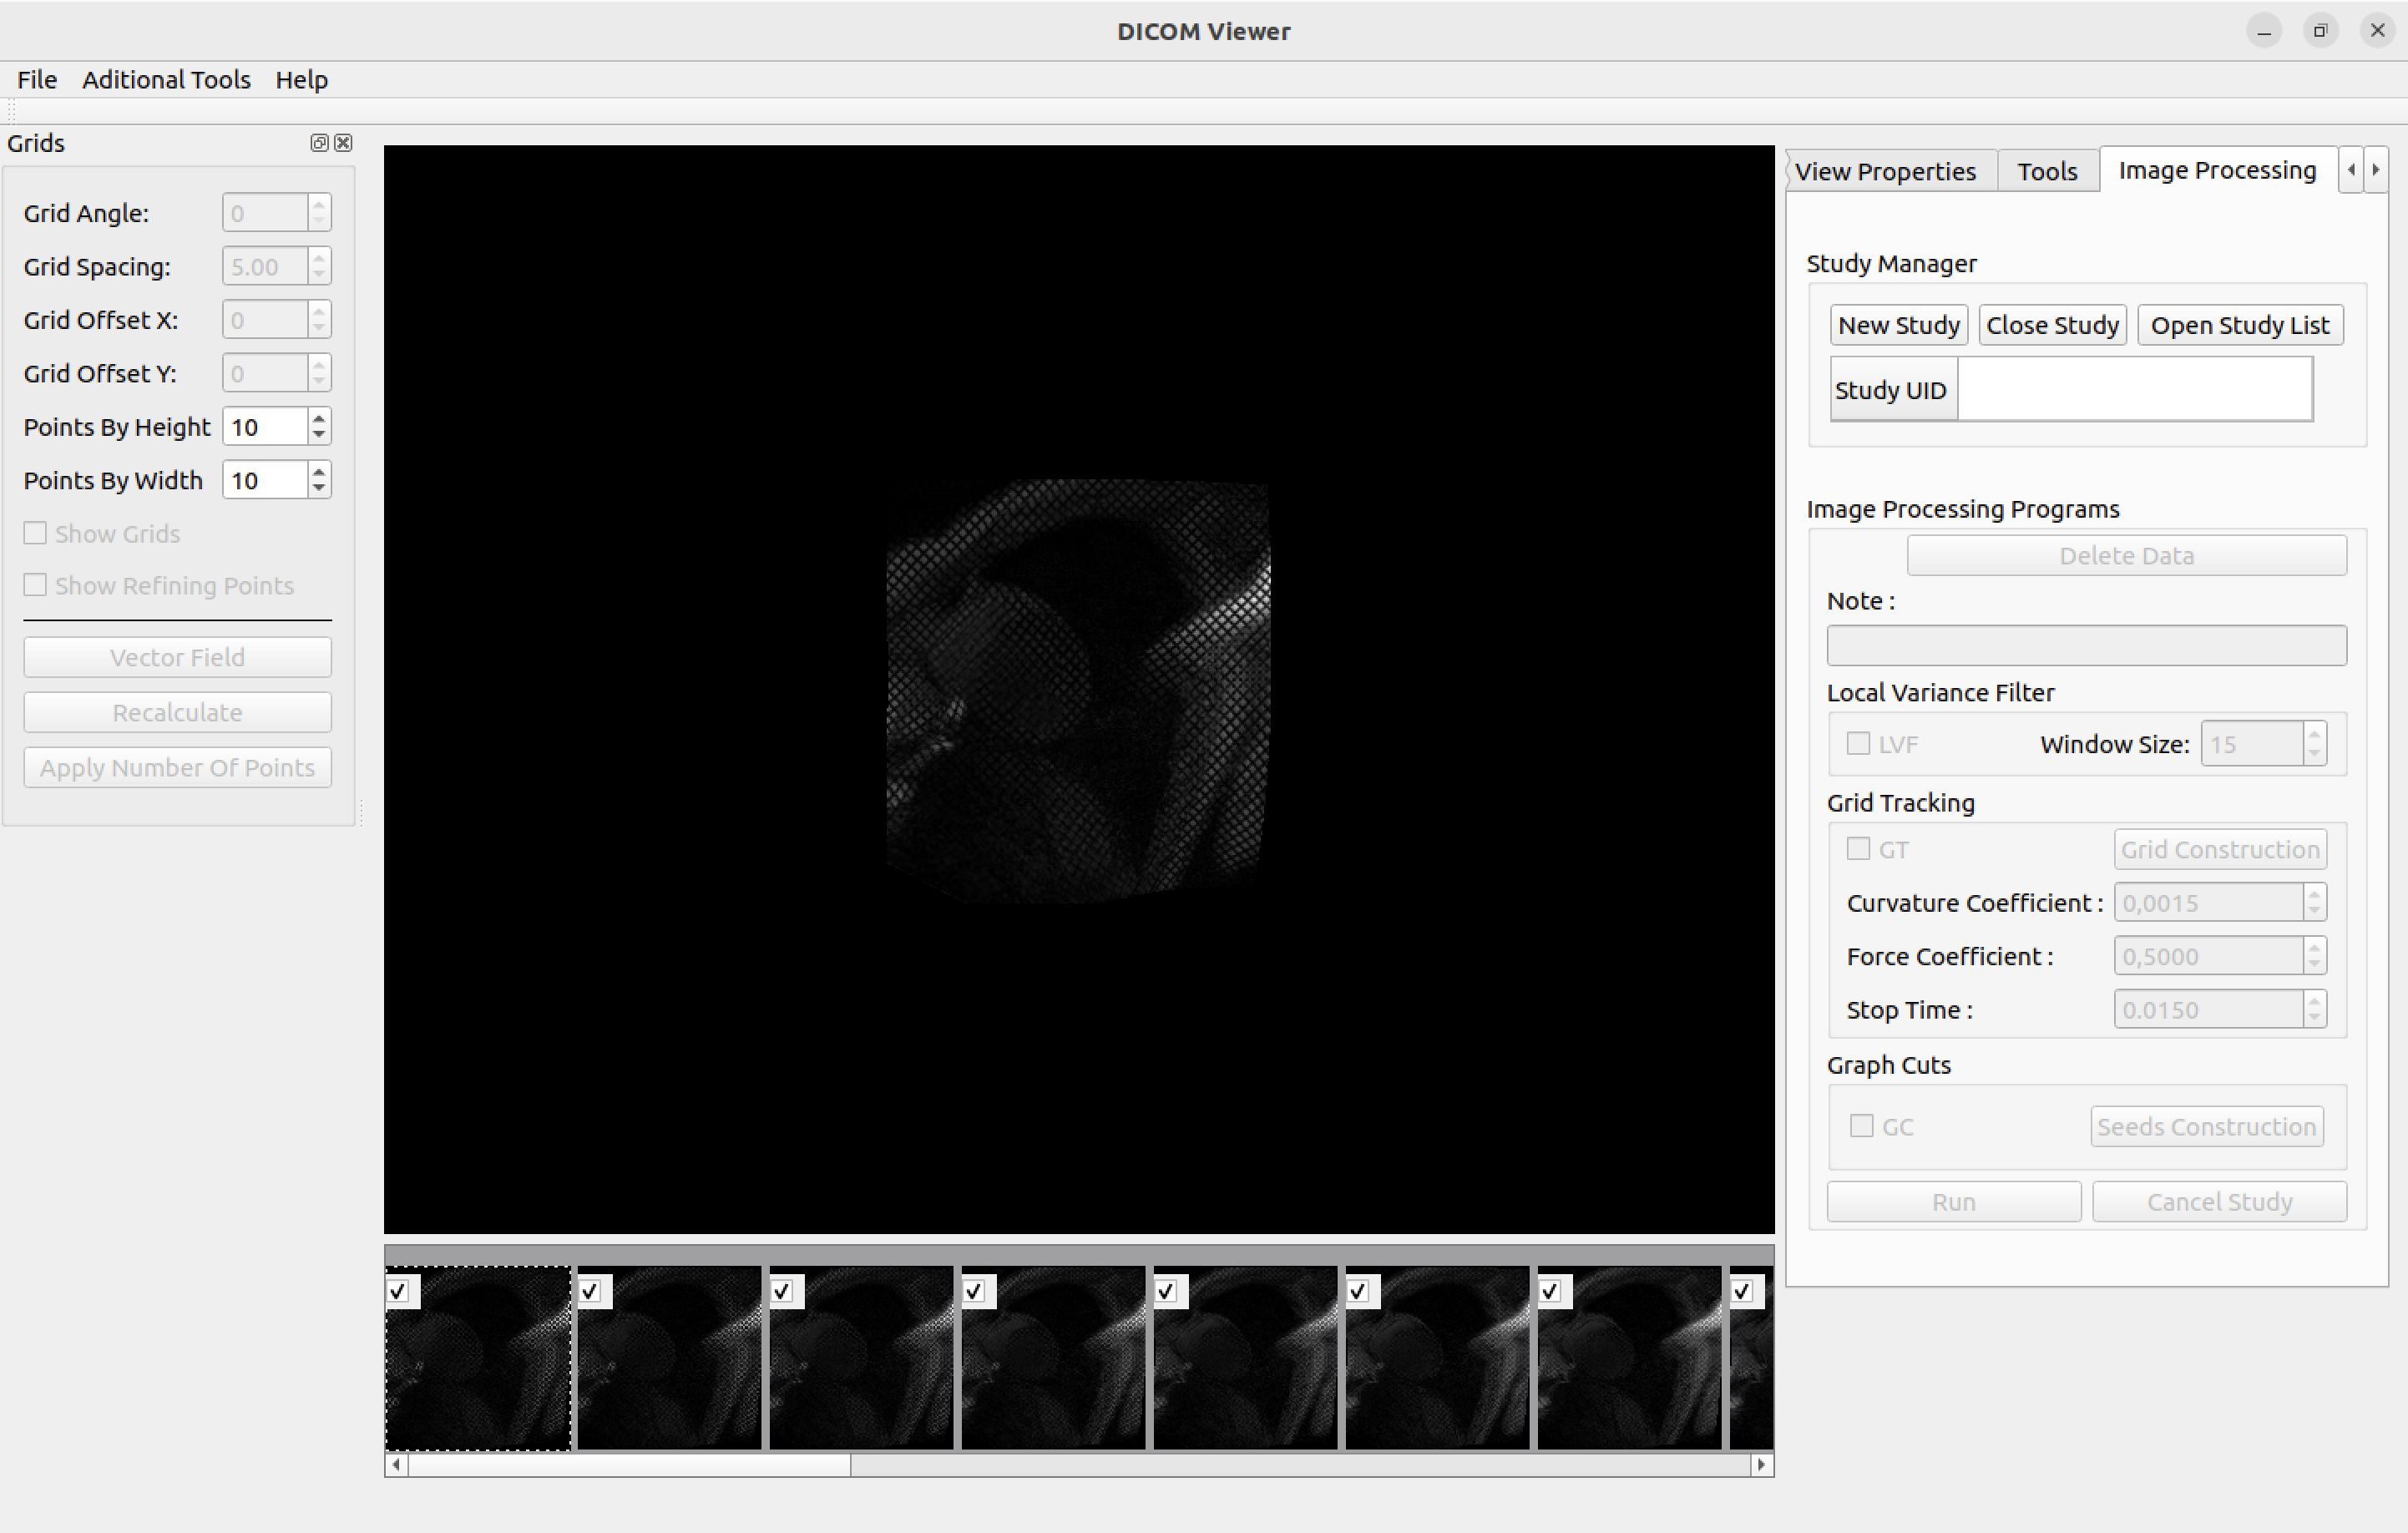
\includegraphics[height=7cm]{media/existing_app/app_with_grids_panel.png}
        \captionsetup{justification=centering}
        \captionof{figure}[Zobrazenie prvej snímky v DICOM Viewer aplikácii]{Zobrazenie prvej snímky v DICOM Viewer aplikácii}
\end {center}

\clearpage

Po zobrazení ľavého postranného panelu sa odhalí celková štruktúra používateľského rozhrania aplikácie.
Tú môžeme rozdeliť na ľavý a pravý postranný panel, medzi ktorými sa nachádza čierna plocha zobrazujúca vybranú snímku. Pod touto snímkou sú zobrazené náhľady všetkých snímok.

Obsahom čiernej plochy, ktorá je dominantná v zobrazení aplikácie, je aktuálne vybraná DICOM snímka. Nad ňou môže byť tiež vykreslená používateľom definovaná mriežka. Náhľady všetkých snímkov, ktoré sa zobrazujú pod aktuálne vybranou snímkou, obsahujú taktiež zaškrtávacie políčko. Toto políčko reprezentuje možnosť, či má byť daný snímok spracovaný v rámci daných 3 podprogramoch.

Obsah pravého postranného panelu je rozdelený na nasledovné karty: \uv{View Properties}, \uv{Tools}, \uv{Image Processing} a \uv{History}.

\begin {center}
        \centering
        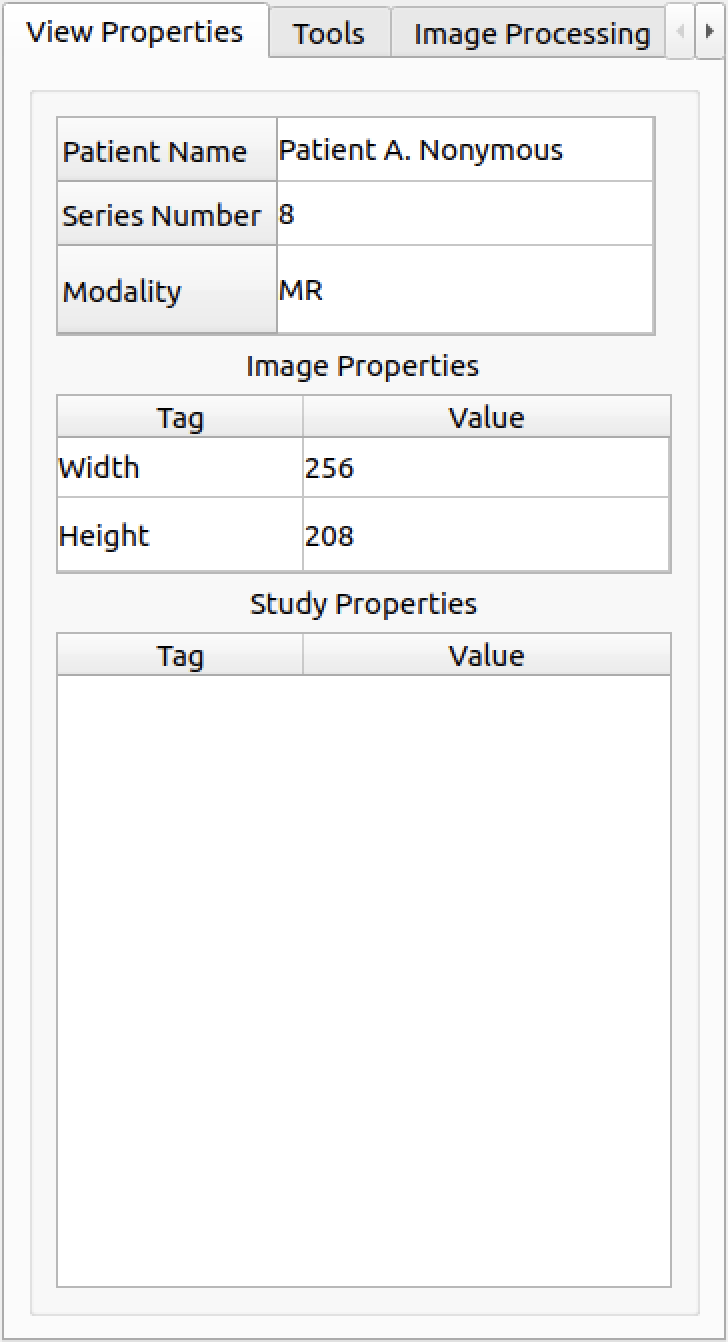
\includegraphics[height=7cm]{media/existing_app/tabs/view_properties.png}
        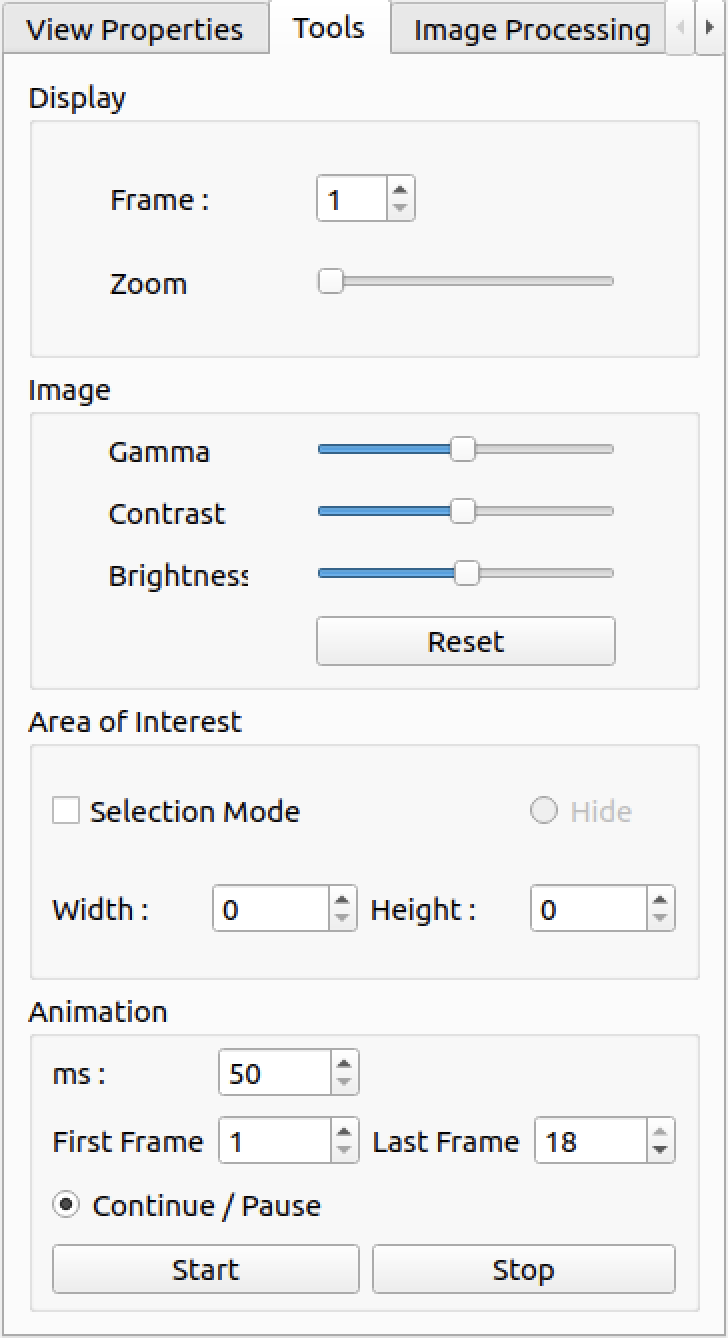
\includegraphics[height=7cm]{media/existing_app/tabs/tools.png}
        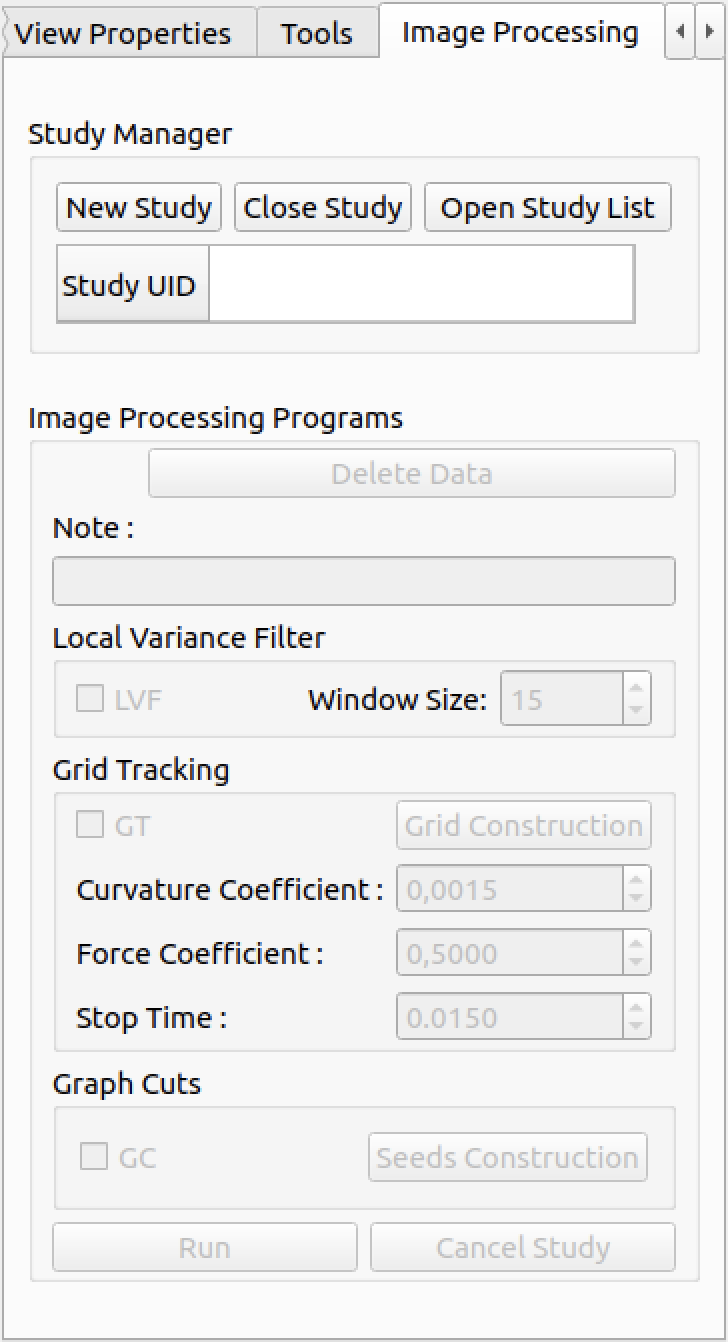
\includegraphics[height=7cm]{media/existing_app/tabs/image_processing_inactive.png}
        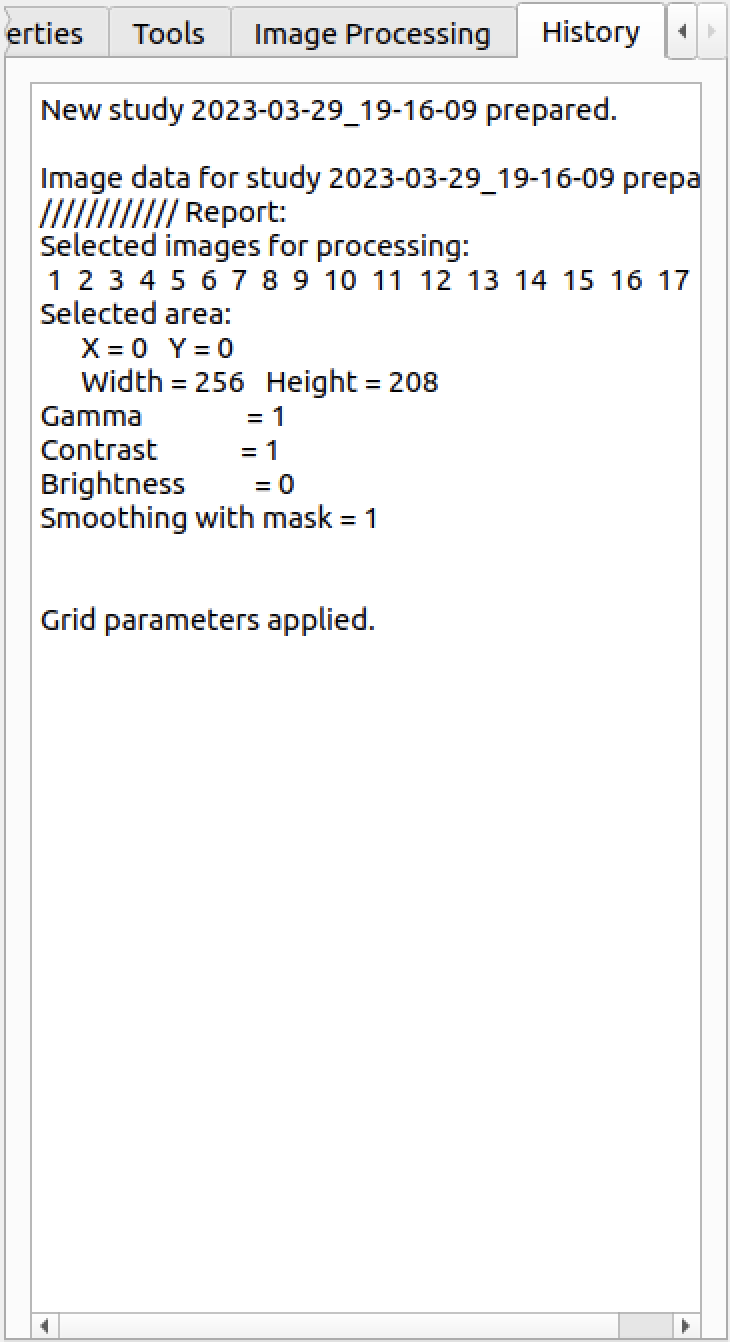
\includegraphics[height=7cm]{media/existing_app/tabs/history.png}
        \captionsetup{justification=centering}
        \captionof{figure}{Zobrazenie obsahu kariet na pravom postrannom paneli}
\end {center}

\uv{View Properties} karta nie je interaktívna -- zobrazuje informácie ako meno subjektu so zobrazenou snímkou, číslo série a modalitu snímkov. Taktiež je zobrazená výška a šírka aktuálne zobrazeného snímku.

Narozdiel od predchádzajúcej karty, \uv{Tools} karta obsahuje interaktívne prvky, ako napr. zobrazenie a zmena indexu zobrazeného snímku, či slider pre priblíženie snímku. Samotnému snímku je možné tiež zmeniť kontrast, jas a gammu pomocou sliderov. Nasleduje sekcia pre nastavenie  oblasti záujmu, pri ktorej je možné nastaviť jej zobrazenie alebo zmeniť jej výšku/šírku -- oblasť záujmu je na základe týchto nastavení vykreslená nad snímkou. Keďže aplikácia podporuje prehrávanie snímkov ako animáciu, aplikácia ponúka nastavenie jej rýchlosti v milisekundách (čo predstavuje čas, ktorý ubehne zobrazením jednej snímky), nastavenie počiatočnej snímky, od ktorej sa animácia spustí, a poslednej snímky, po ktorú animácia bude spustená. Okrem nastavenia parametrov animácie nesmú chýbať tlačidlá pre samotné spustenie a zastavenie animácie.

Na ďalšej karte \uv{Image Processing} sa nachádzajú tlačidlá ovládajúce manažéra štúdií. Tento \uv{manažér} zoskupuje rôzne štúdie, pod ktorými sa ukladajú rôzne parametre aplikácie. Po kliknutí na tlačidlo \uv{Open Study List} sa zobrazí nové okno so všetkými štúdiami a ich parametrami.
Pre interakciu s ostatnými poliami na tejto karte je potrebné najprv vytvoriť novú štúdiu kliknutím na tlačidlo \uv{New Study}. \newline Štúdiu je tiež možné ukončiť zvolením tlačidla \uv{Close Study}. Každá štúdia je reprezentovaná jedinečným ID, ktoré sa skladá z dátumu a času jej vytvorenia.
Vytvorením novej štúdie sa aktivujú polia \uv{Image Processing Programs} sekcie. Táto sekcia ponúka tri hlavné začiarkavacie políčka -- prvé reprezentuje spustenie aplikovania filtra lokálnej variancie. Druhé z nich reprezentuje spustenie algoritmu pre zarovnanie vygenerovanej mriežky s mriežkou myokardu vytvorenou pomocou SPAMM techniky a tretie spustenie algoritmu segmentácie srdečných komôr pomocou grafových rezov. Zaškrtnutím daného políčka a kliknutím na tlačidlo \uv{Run} sa algoritmus príslušný danému políčku spustí. Pre \uv{Grid Tracking} algoritmus je v tejto sekcii možné definovať tri parametre, a to \uv{Curvature Coefficient}, \uv{Force Coefficient} a \uv{Stop Time} (viď \ref{helper_apps}).

Účelom poslednej karty \uv{History} je výpis rozličných záznamov pre informovanie používateľa o prebiehajúcich krokoch aplikácie. \clearpage

Obsah ľavého postranného panelu sa mení v závislosti na zvolenej možnosti z menu Aditional [sic] Tools. Momentálne sa zobrazuje obsah ľavého panelu po zvolení možnosti \uv{Grid Tools}. V paneli je možné nájsť nasledujúce nastavenia:

\begin {itemize}
\item {Grid Angle -- nastavuje uhol mriežky,}
\item {Grid Spacing -- nastavuje rozpätie jednotlivých bodov,}
\item {Grid Offset X -- $x$ pozícia od ľavého horného bodu,}
\item {Grid Offset Y -- invertovaná $y$ pozícia od ľavého horného bodu,}
\item {Points by Height -- udáva počet bodov na úsečku mriežky na výšku,}
\item {Points By Width -- udáva počet bodov na úsečku na šírku,}
\item {Show Grids -- indikuje, či má byť zobrazená mriežka,}
\item {Show Refining Points -- indikuje, či majú byť zobrazené body, ktoré upresňujú pozíciu mriežky,}
\item {Vector Field -- spočíta rozdiel v pohybe mriežky medzi predchádzajúcou a aktuálnou snímkou,}
\item {Recalculate -- odošle dáta \texttt{grid-tracker} podprogramu pre opätovné zarovnanie mriežky voči SPAMM mriežke,}
\item {a Apply Number of Points -- uloží mriežku ako textový TNL multivektor.}
\end {itemize}

Ostatné dve možnosti z menu \uv{Aditional [sic] Tools} nie je potrebné pre účely tejto práce popisovať.